\subsection{Ring configurations}

The key property of rings is that they seperate a planar graph $G$ into an exterior $M$, a border ring $R$ and an interior $\core$. The concept of a ring $R$ and its interior $\core$ will be used so often that we give it a well-known name.

\begin{definition}
    A planar graph $\confg = R_n + \core$ consisting of a ring $R_n$ and an interior $\core$ is called a \emph{ring configuration} on $R_n$. $\core$ is called the \emph{core} of $\confg$.
\end{definition}

\begin{figure}[!ht]
    \centering
        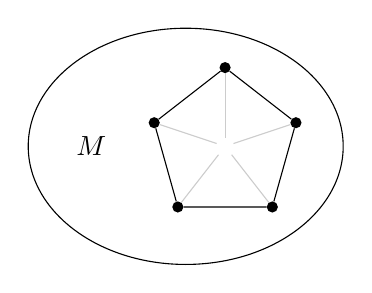
\begin{tikzpicture}
        \draw[fill=white] (-0.5, 0) ellipse (2cm and 1.5cm);
        %\draw[fill=lightgray, draw=black] (0,0) circle (1.25cm);
        %\draw[fill=white] (0,0) circle (0.75cm);
        \node at (-0.7, 0.9) {$\confg$};
        \node at (-1.7, 0) {$M$};

        \node[inner sep=1mm] (c) at (0, 0) {$\core$};
        \node[circle, fill, scale=0.015cm] (l1) at (0, 1) { };
        \node[circle, fill, scale=0.015cm] (l2) at (0.9, 0.30) { };
        \node[circle, fill, scale=0.015cm] (l3) at (0.6, -0.77) {};
        \node[circle, fill, scale=0.015cm] (l4) at (-0.6, -0.77) {};
        \node[circle, fill, scale=0.015cm] (l5) at (-0.9, 0.30) {};

        \draw[opacity=0.2] (c) -- (l1);
        \draw[opacity=0.2] (c) -- (l2);
        \draw[opacity=0.2] (c) -- (l3);
        \draw[opacity=0.2] (c) -- (l4);
        \draw[opacity=0.2] (c) -- (l5);
        \draw (l1) -- (l2) -- (l3) -- (l4) -- (l5) -- (l1);
    \end{tikzpicture}
    \caption{The graph $G=M + \confg$ that contains the configuration $\confg=R_5 + \core$.}
\end{figure}

The idea of $k$-reducibility is that we try to find a \textit{common ring coloring} for $M+R$ and the configuration $\core+R$. If two such colorings can be found, then we can combine both colorings to color $G$. This is exactly a more general approach to what we did for the five color theorem, where the configuration was the vertex $v$ with five neighbors.

Because we allow $M$ and $\confg$ to be arbitrary, we might not always be guaranteed to find a common ring coloring. To obtain certainty, we must have some control over the colorings on both sides. We can obtain this control by adding extra vertices on the other side of the ring in $M+R$ and $\core+R$. Consider the following two graphs.

\begin{figure}[!ht]
    \centering
    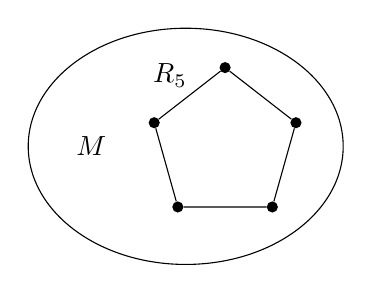
\begin{tikzpicture}
        \draw[fill=white] (-0.5, 0) ellipse (2cm and 1.5cm);
        \node at (-1.7, 0) {$M$};
        \node at (-0.7, 0.9) {$R_5$};

        \node[circle, fill, scale=0.015cm] (l1) at (0, 1) { };
        \node[circle, fill, scale=0.015cm] (l2) at (0.9, 0.30) { };
        \node[circle, fill, scale=0.015cm] (l3) at (0.6, -0.77) {};
        \node[circle, fill, scale=0.015cm] (l4) at (-0.6, -0.77) {};
        \node[circle, fill, scale=0.015cm] (l5) at (-0.9, 0.30) {};

        \draw (l1) -- (l2) -- (l3) -- (l4) -- (l5) -- (l1);
    \end{tikzpicture}
    \hspace{1cm}
    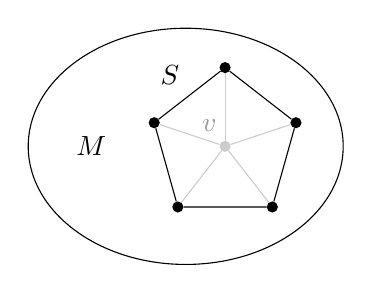
\begin{tikzpicture}
        \draw[fill=white] (-0.5, 0) ellipse (2cm and 1.5cm);
        \node at (-1.7, 0) {$M$};
        \node at (-0.7, 0.9) {$S$};

        \node[opacity=0.4] (c) at (-0.2, 0.27) { $v$ };
        \node[circle, fill, scale=0.015cm, opacity=0.2] (c) at (0, 0) {};
        \node[circle, fill, scale=0.015cm] (l1) at (0, 1) { };
        \node[circle, fill, scale=0.015cm] (l2) at (0.9, 0.30) { };
        \node[circle, fill, scale=0.015cm] (l3) at (0.6, -0.77) {};
        \node[circle, fill, scale=0.015cm] (l4) at (-0.6, -0.77) {};
        \node[circle, fill, scale=0.015cm] (l5) at (-0.9, 0.30) {};

        \draw[opacity=0.2] (c) -- (l1);
        \draw[opacity=0.2] (c) -- (l2);
        \draw[opacity=0.2] (c) -- (l3);
        \draw[opacity=0.2] (c) -- (l4);
        \draw[opacity=0.2] (c) -- (l5);
        \draw (l1) -- (l2) -- (l3) -- (l4) -- (l5) -- (l1);
    \end{tikzpicture}
    \caption{On the left, a graph $M+R_5$ without extra vertices. On the right, a graph $M+S$ where $S=R_5+v$. The graph $S$ is called a \textit{reducer}.}
    \label{fig:reducertut}
\end{figure}

The colorings of the ring in $M+R_5$ can be any 3-coloring or 4-coloring depending on $M$. However, in the graph $M+S$ it is not possible the color the ring in four colors. Due to the extra vertex introduced by $S$, we are guaranteed to find only 3-colorings on the ring regardless of $M$. An example of such a 3-coloring is $cabab$.

This guaranteed 3-coloring is key information in the reducibility proof of $R_5$. Therefore, let us instead reduce the graph $G=M+R+\core$ to

\begin{equation}
    M+S \;\;\text{and}\;\; \core+S' \quad \text{with} \quad R \subset S,S'.
\end{equation}

For both reducers $S$ and $S'$, we require that $|S-R| \leq k$. Here $k \geq 0$ is a limit on the amount of extra vertices we can add. Ideally, of course, we want $k=0$ such that we reduce the size of $G$ as much as possible. By increasing $k$, we get a smaller size reduction of $G$ in exchange for more control over the colorings.

\begin{itemize}
    \item If $k=0$, then $S=R$ and we reduce to $M_1+R$ and $\core+R$. This is the smallest possible reduction and ideal situation.
    \item If $k=1$, then we can set $S=R+v$ like in Figure \ref{fig:reducertut}. Our reduced graph is then one vertex larger.
    \item If $k = |\confg|$, then we can set $S = \confg$ and $S' = R$ such that we obtain $M+\confg$ and $\confg$. Clearly, they have a common ring coloring, but we did not achieve any reduction in size with $M+\confg = G$. 
\end{itemize}

Therefore, to obtain a reduction in size, we should also require that $k < |\confg|$. We are now ready to define this concept of reducibility.

\begin{definition}
    A configuration $\confg=\core+R$ is \emph{$k$-reducible} if for all planar graphs $G=M+\confg$ and some reducers $S$ and $S'$ on $\leq k < |\confg|$ vertices, there exists a common ring coloring for $M+S$ and $\core+S'$.
\end{definition}
\begin{definition}
    The ring $R_n$ is \emph{$k$-reducible} if all configurations $\confg$ on $R_n$ are at most $k$-reducible.
\end{definition}

A trivial example is the 0-reducibility of the rings $R_1, R_2$ and $R_3$. The only possible colorings on these rings are of the form $ a, ab$ and $ abc$ respectively. This means that any two colorings of $M+R$ and $\core + R$ are of this same form and therefore equal. You might say that the colorings $abab$ and $acac$ are different, but we can make them equal by renaming the color $b\rightarrow c$. We consider two colorings that have this property to be \textit{equal}.

\begin{definition}
    \label{def:coleq}
    Two colorings $x$ and $y$ are \emph{equal} if they differ only by a renaming of the colors $a,b,c$ and $d$. 
\end{definition}

Next, we move on to Kempe-chains.
